\documentclass{report}
\usepackage[utf8]{inputenc}
\usepackage{graphicx}
\usepackage{a4wide}
\usepackage{url}

\title{Blockchain Based E-Voting System}

\begin{document}


\begin{center}

\textup{\large {\bf\emph{A Project Report On}}}

\vspace{0.3in}
\LARGE {\textbf {Blockchain Based e-Voting System}}


\vspace{0.5in}
\small \emph{\large{A dissertation submitted by}}

\vspace{0.1in}
{\large{\bf Anjali Sharma \\ (17/MAM/003)}}

\vspace{0.4in}
\emph{\large{In the partial fulfillment of the requirements of the degree of Master of Science in Applied Mathematics}}

\vspace{0.4in}
\emph{\large {Under the supervision of}}

\vspace{0.1in}
{\textbf{\large {Dr. Amit Awasthi}}}

\vspace{0.5in}

\includegraphics[width=0.35\textwidth]{48383172_349071859220901_5141705199164850176_n.jpg}

\vspace{0.3in}
\bf
\large {{Department of Applied Mathematics}\\ {Gautam Buddha University, Greater Noida, India}}

\vspace{0.1in}
\today
\end{center}
 \onehalfspacing


 \newpage
 \begin{center}
\section*{Declaration}
 \end{center}
 I undersigned hereby declare that the work which is being represented in this dissertation entitled \textbf{“Blockchain Based e-Voting System”} is submitted for the partial fulfillment of the degree of M.Sc. in Applied Mathematics, Department of Applied Mathematics, Gautam Buddha University, Greater Noida, India. It is an authentic record of my work carried out under the supervision and the guidance of \textbf{Dr. Amit Awasthi}, Assistant Professor, Department of Applied Mathematics, Gautam Buddha University.  I have followed ethics to the best of my knowledge. No part of this project has been submitted for the degree of any other academic qualification at any other university or examination body in India or abroad.

 \vspace{1.0in}
 
 Date:- \hfill Anjali Sharma 
 
 \vspace{0.1in}
 Place:- 

 
\newpage
 \begin{center}
\section*{Certificate}
 \end{center}
This is to certify that this dissertation entitled \textbf{“Blockchain Based e-Voting System”} being submitted by \textbf{Ms. ANJALI SHARMA (17/MAM/03)} to Department of Applied Mathematics, Gautam Buddha University, Greater Noida, India for the partial fulfillment of the degree of master of science in Applied Mathematics, is a record of the work carried out by him. He has worked under my supervision and has fulfilled the mandatory requirements for the submission of this dissertation. To the best of my knowledge, the results contained in this dissertation have not been submitted in part or full to any other University/ Institute/ Organization for the award of any degree/ diploma. 

 \vspace{1.0in}
 
 Date:- \hfill Dr. Amit Awasthi
 
 \vspace{0.1in}
 Place:- \hfill HOD\\
 \null \hfill Department of Applied Mathematics\\
\null \hfill Gautam Buddha University\\
\null \hfill Greater Noida, India.


 \newpage
 \begin{center}
\section*{Acknowledgements}
 \end{center}
I wish to express my gratitude to a lot of people for guiding and helping me in my M.Sc. dissertation Project. I would never have been able to complete my dissertation without their guidance. I shall begin by thanking my supervisor Dr. Amit Awasthi for his kind supervision and support to complete the work. His enthusiasm, encouragement and faith in me throughout have been extremely helpful.\\
I would like to thank Prof. N.P. Melkania, Dean, School of Vocational Studies and Applied Sciences for his moral support and encouragement. 
 I would like to thank my Parents and my friends Bhavna, Niharika, Shalu, Payal and Shrishti for their assistance and motivation. It wouldn’t have been possible without their support. \\
Last but not the least, I would like to thank Gregory for his amazing tutorials that made this journey enjoyable.
\\
The study has indeed helped me to explore more knowledge avenues related to my topic and I am sure it will help me in my future.

\vspace{1.0in}
 
 Date:- \hfill Anjali Sharma 




\tableofcontents
\pagebreak
\textbf{Abstract:}
Blockchain Technology has emerged as a key technology that will modify the way in which we share information. Building trust in distributed environments without the need for authorities is a technological advance that has the potential to change many industries.
Building an electronic voting machine that meets the social, economic and legal requirements of voting procedure. Blockchain is a secure and reliable technology that has infinite prospects in the world of information technology, by making it possible to create tamper-proof digital platform for storing and sharing data. In this paper we address voters privacy concern, the authenticity of the voting process using Blockchain technology and standard. ECDSA to achieve voter's anonymity. This paper evaluates the potential of distributed ledger and implementation of this to improve security and prudentiality.\\
\\
\textbf{Keywords:} Blockchain, ECDSA, Electronic Voting, Distributed Ledger, Cryptosystem

\chapter{Introduction}
Voting is a fundamental right of every citizen. It enables them to choose the leaders of tomorrow. Voting not only enables the citizens to vote for political parties, but it also helps them to realize the importance of citizenship. Many people do not vote thinking one vote will not make a change, but as a matter of fact, it does. A nation’s political foundations are built using elections.\cite{blais1999people}   Elections in the Republic of India constitution include elections for the Parliament, Rajya Sabha, Lok Sabha, the Legislative Assemblies, and numerous other Councils and local bodies. EVMs were manufactured in 1989-1990 and were used for the first time in 16 assembly constituencies -- 5 in Madhya Pradesh, 5 in Rajasthan, and 6 in Delhi elections to the respective legislative assemblies in November 1998. Before this paper ballots were used for the election process. United States of America still practises using paper ballots. Electronic voting machines have been viewed as flawed, by the security community, primarily based on physical security concerns. Anyone with physical access to such machine can sabotage the machine, thereby affecting all votes cast on the aforementioned machine.\cite{hjalmarsson2018blockchain} Blockchain technology originates from the  architectural design of the cryptocurrency. S. Nakamoto's work on Bitcoin \cite{nakamoto2008bitcoin} prompted considerable research on blockchain technology.  It is a strong database platform, with strong consistency support. It is a distributed and decentralized , computation and information sharing platform that enables multiple authoritative domains, who donot trust each other, to cooperate, coordinate and collaborate in a rational decision making process. It is " an open, distributed ledger that can record transaction between two parties efficiently in a verifiable and permanent way.\cite{iansiti2017truth}" Here we are using a modified version of blockchain technology for the purpose of a secure decentralised storage. \\
\\
\textbf{Literature Review}
\begin{enumerate}
    \item Oswald, 2002 :  This paper provides the application of elliptic curves in cryptography. It provides a general idea of elliptic curve cryptography by basic abstract algebra and elementary number theory. It also gives an idea of Elliptic Curve Digital Signature Algorithms.

\item Nakamoto, 2008:  This paper provides a peer-to-peer version of electronic cash transfer online directly from one party to another without a third party for validation. It provides a solution of double-spending problem through a peer-to-peer network.

\item Veerman, 2010: This paper explains the mathematics behind elliptic curve cryptography. It thoroughly discusses public key cryptosystems (PKC), Elliptic
curve cryptosystems and how they are linked to the discrete
logarithm problem (DLP). 

\item Agarwala, 2014: In this paper electronic voting machines used in Indian election are exclusively examined. It provides a 
description of the machine’s design and operation in detail. 
It throws a light on the serious attacks that can alter election results and
violate the secrecy of the ballot. 

\item Þ. Hjálmarssonr & K. Hreiðarsson, 2018: In this paper an electronic voting system using distributed ledger technologies is built. The paper elicitates the requirements of building electronic voting systems and identifies the legal and technological
limitations of using blockchain. Also this paper evaluates the potential of distributed ledger technologies
through the election process. 



\end{enumerate}
\section{Preliminaries}
 Transparent, secure and accurate voting systems are the key features of democracy. For some nations, automated elections mean that people can trust the results because it allows for a process that is auditable and reduce human error. For other countries, particularly large ones like Brazil, India and the Philippines, electronic voting and electronic counting means that people can get official election results within hours, instead of weeks. \\
Also it is vitally important that everyone who is eligible, to participate in elections. Electronic voting paves a way to make voting more accessible and thus allows disable people to vote independently.
One of the reasons electronic voting system has been praised so highly is that it’s designed around the idea that all parties, citizens and election commissions are able to audit the electoral process at every stage. The voting machines print a paper receipt every time a vote is registered electronically. This makes it easy to perform recounts and audits because you can compare the electronic count with the paper count.\cite{WinNT7}
To secure end-to-end verifiable e-voting system we need a cryptographic technique for authenticated end-to-end verification secret ballot election. Voters should receive assurance that their votes cast as intended recorded as cast and tallied as recorded. End-to-end verifiable refers to two properties. \\
1. Each voter is able to identify or verify if there vote would have been cast as intended and recorded as cast. \\
2. Anyone can verify if all votes are tallied as recorded. Also old traditional voting depends on trustworthy individual at the polling station that leading to the introduction of automatic paper less secure e voting system.


Our methodologies drive efficiencies into every stage of the election process. We make voter registration faster and more accurate. We also speed up voter authentication, preserve voter secrecy, and make the storage, counting and transmission of votes 100$ \% $ secure.\\
\\
\textbf{Contribution} We have tried to construct a simple voting application that uses ECC techniques and blockchain technology. We have also provided our theoretical picture of realtime blockchain voting that is secured from double voting.

\section{Digital Signature}
 Once a culture reaches to a sophistication of  science and language the demand for Secret symbolic communication  flourishes. For decades it has been used in diplomacy militancy and espionage . Due to modern technology, now Cryptography is an essential tool for banking and personal privacy. The Classic Cryptography that used just pen and paper began in early 20th century.  Clay tablets from Mesopotamia were meant to protect information, one dated near 1500 BC had craftsman's encrypted recipe for pottery glaze.\\

     \begin{figure}[!h]
    \centering
     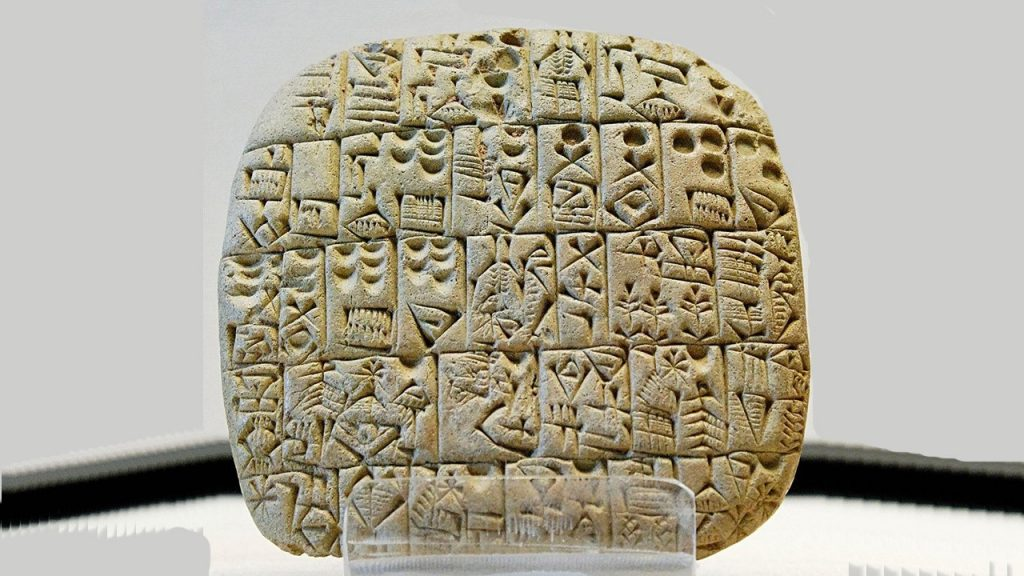
\includegraphics[scale=0.12]{Ancient-clay-tablet-1024x576.jpg}
     
\includegraphics[scale=0.76]{3c60b59d-9a9b-453d-9897-8cc601e3d67f_l.jpg}
\caption{Ancient methods of Cryptology}
  \end{figure}
  
   In ancient Greek a device called Skytale which is now known as Skytale transposition cypher was used.  The most modern breakthrough was the invention of Telegraph and radio which could send and receive messages  instantly. The morse code was then developed by Samuel Morse. Thus cryptography became a major tool for sending and receiving classified information. The onset of world war 1 and world war 2 led to major developments in the field of cryptography due to constant encryption and subsequent decryption. \\
The word crypto means hidden or secret. The word cryptography origins from the combination of cryptograph and crytoanalysis. A cryptograph is an encrypted message. The study of these encrypted messages, ciphers and cryptosystems with the aim of understanding how they work and improving techniques for defeating or weakening them is called cryptoanalysis. It is the study of analyzing information system in order to study the hidden aspects of the systems.

The discrete logarithm problem is considered to be computationally intractable. That is, no efficient classical algorithm is known for computing discrete logarithms in general.
For any group G, denote its group operation by multiplication and its identity element by 1. Let b be any element of G. For any positive integer k, the expression bk denotes the product of b with itself k times. There are groups for which computing the discrete logarithm is nearly impossible.
There are two types of discrete logarithm cryptography, finite field and elliptic curve. \\
 Finite field is useful for Cryptography because its arithmetic properties allow it to be used for scrambling and descrambling of data. FFC is a public key Cryptography method using operations in a multiplicative group of finite field. in order to use FFC both pairs have to share some domain parameters. 

\subsection{Digital Signature}
 A digital signature is a mathematical scheme for verifying the authenticity and legitimacy of digital messages or documents.  A valid digital signature shows the recipient that the message is authenticated and also the sender cannot deny having sent the message.  It also ensures the integrity of the message that it was not altered during transit.  Digital signatures are based on asymmetric Cryptography and provide validation and security to messages sent through a non secure channel.  In 1976, Whitfield Diffie and Martin Hellman first described the notion of a digital signature scheme, but they only gave a theoretical conjecture based on trap door functions.  In 1977, Ronald Rivest, Adi Shimir and len adelman invented the RSA algorithm which produced the primitive digital signature. The RSA scheme applies sender's  private key to a message to generate a signature.  This could then be verified by applying the corresponding  public key to the message and signature,  providing either a valid  or invalid  result. Thus it fulfills the verification requirements of the digital signature. Then in 1985 Neal Koblitz and Victor Miller  independently suggested the use of elliptic curve in Cryptography. Thus introducing elliptic curve to the world of cryptography
\subsection{Elliptic Curve}
In general elliptic curves combines number theory and algebraic geometry. These curves can be defined over any field of numbers (i.e., real, integer, complex and even $F_p$).
 The standerd equation of elliptic curve over an algebraic field is of the form
$$ y^{2}=x^{3}+ax+b$$
  
  It is a combination of algebraic properties with graphical technique .
The set of all of the solutions to the equation forms the elliptic curve. Changing a and b directly changes the shape of the curve. Small changes in these parameters often result in major changes in the set of (x, y) solutions.
    Elliptic curves offer more efficient implementations and bandwidth advantages with respect to shorter signatures and keys at the same security level as e.g. RSA. In terms of numbers, about 160-256 bit vs. 1024-3072 bit. For elliptic curves, a security level of 80 bit provides medium-term security but bit lengths up to 256 bit are usually used, which corresponds to a security level of up to
128 bit.
\subsubsection{Elliptic curves as Sets}
Let K be a field, and K' its algebraic closure. An elliptic curve $E \subset P^2(K')$ is a non-singular, projective curve given by an equation of the form
$$y^2+a_1xy + a_3y = x^3 + a_2x^2 + a_4x + a_6$$
with all ai $\in$ K'. An equation of this form is known as Weierstrass equation. 
 We will sometimes write $E/K$ if we want to stress the field K.
When the characteristic of K does not equal 2 or 3, we can rewrite the Weierstrass equation to
$$y^2 = x^3 + Ax + B$$
with A, B $\in$ K . Most of the time we will work in fields of characteristic $\neq$ to 2 and 3.
Although elliptic curve is represented by this equation,it is a projective curve. It always has exactly one point on the line at infinity,which is O = [0 : 1 : 0].\\
To check if the curve defined by the Weierstrass is nonsingular, we compute the discriminant $\delta$, which is $−16(4A^3 + 27B^2)$ when char(K') $\neq$ 2, 3. When E is defined over K, we define E(K) to be the set of K-rational points of E. That is, the subset of E, consisting of points with coordinates in K. Hence $E(K) \subset P^2(K).$ \cite{stinson2005cryptography}
\subsubsection{Elliptic curves over a finite field}
Let $K = F_q$ be a finite field with q elements in a elliptic curve defined on K. As we know the sheer complexity of computing a precise number of rational points of an elliptic curve E over K, this is where the Hasse's theorem emerges. It provides an estimate of the number of points on an elliptic curve over a finite field such that both upper bound and lower bound exist. \cite{veerman2010elliptic}
Further the Helmut Hasse's result states that on a finite field with q elements with
N = Number of points on the elliptic curve, we can state that
$$ |N-(q+1)|\leq 2{\sqrt q}$$
Hence we can say that the number of points on the elliptic curve is proportional to the number of elements in the field.\\
Elliptic curves on finite fields is generally used for factorization of large integers. The group structure on the points of the elliptic curve is the crucial reason behind it. For example the group of invertible elements in finite fields, $F^*_q$, can  be applied to the group of points on an elliptic curve i.e the discrete logarithm. The group structure of elliptic curves is generally more complicated. The reason behind this is that choosing an elliptic curve allows more compatibility than choosing the value of q. 

\subsubsection{Elliptic curve cryptography}
Elliptic-curve cryptography is a public-key cryptographical system based on algebraic structure of elliptic curves over finite fields. It requires smaller keys compared to several other non-Elliptic curve cryptography system to provide equal security. The size of the elliptic curve also ascertains the difficulty of the system. \cite{andrea}
For elliptic-curve-based protocols, we can certainly say that even with a known base value, finding the discrete logarithm of a random elliptic curve element is nearly infeasible. The security of this system depends on the ability to compute a point multiplication and the inability to compute the original values. The U.S. National Institute of Standards and Technology endorses elliptic curve cryptography algorithms, specifically elliptic curve Diffie–Hellman \cite{maurer2000diffie} (ECDH) for key exchange and Elliptic Curve Digital Signature Algorithm (ECDSA) for digital signature. We will discuss ECDSA further in our project.\cite{koblitz1987elliptic}
\subsubsection{Diffie-Hellman and ElGamel over elliptic curve}
Elliptic-curve Diffie-Hellman (ECDH) is an anonymous, zero knowledge key agreement protocol. This protocol allows two parties, each having a public key and a private key, to generate a private conversation over an insecure channel. This can be further used as a key or it can be further used to derive any another key. This secret key, can then be used to encrypt subsequent database or secret conversation using a symmetric-key cipher or any other subsequent hash.\\ \cite{brown2009standards}
Adjusting the ElGamal cryptosystem is also not difficult. This protocol derives it's endurance from the Trapdoor function. The discrete logarithm problems can be really unpractical and time-consuming for a given number even when the inverse operation of the power is fairly easy to compute.
\subsection{Review of elliptic curve based signature schemes}
Today, we can find elliptic curves cryptosystems\cite{WinNT20} in major companies of the world. It is also one of the key factors in cryptocurrencies like bitcoin. Thus it plays an major role in IT fields and computer technologies. 


Elliptic Curve Digital Signature Algorithm, is used to create a digital signature of data. It follows the zero knowledge protocol allowing us to verify the authenticity of the data without compromising it's security.
 This digital signature works as any physical signature but cannot  be forged under any circumstance. The difference between an ECDSA signature and a real world signature is that it is not possible to tamper or duplicate an ECDSA signature.
 We have a standard elliptic equation which draws a curve on a graph. We can choose any random point on the curve. Then we compute any random number, this is our Private key, putting these values in a standard equation we obtain a second point on the curve. This is called the Public key.
To sign a data using ECDSA digital signature, we require the Private key and the hash of the data. Substituting this on the Standard equation, we obtain our digital signature. 
The Signature has two parts, (r) and (s). To verify the Signature, we only require the Public key. If we apply the Private key into a specific equation with one part of the signature (s), then if it is signed correctly using the the Private key, it gives us the other part of the signature (r). 
So we can say that a digital signature is valid if we obtain the part (r) using only the Public key and the part (r). The private key is set such that it cannot be guessed and the signature cannot be duplicated using the Public key.
\subsection{The Standard Equation}
\begin{center}
         $y^2 = (x^3 + a * x + b) mod p$
         \end{center}
This is the standard equation in Elliptic Curve cryptography.
The equation applies a modulus operation. The values of $y^2$ lie between 0 and p-1. Therefore there are total p possible values. Since the equation applies only on integers, only a subset of these values N are a perfect square, i.e $N < p$ .
Since we have the square function on y, each x gives two points. There are N/2 possible ‘x‘ coordinates which give a point on the curve. Hence we can conclude that the elliptic curve has a finite number of points. 

\subsection{Point addition}
The Point Addition means by adding a point P to another point Q. If we draw a line from P to Q, it will intersect the curve on a third point. When we take mirror image of that point, we obtain another point, say S
Let us take an equation $y^2 = x^3 - 4x$. This equation is symmetric on the X axis. The point of P+Q point addition is the symmetrical point through the X axis, of the point -S.[2]. As shown in the figure \ref{fig:ptadd}.\cite{WinNT21}
\begin{figure}
 \centering
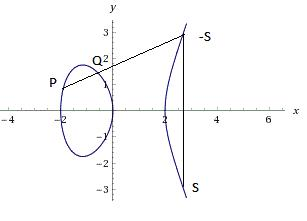
\includegraphics[scale=0.75]{elliptic2.jpg}
    \caption{Point Addition}
    \label{fig:ptadd}
\end{figure}

\subsection{Point Multiplication}
On two elliptic curves we draw a tangent from point P. This tangent intersects the curve at a third point. We take the symmetric point 2P. Multiple additions of the same point repeats same line with the same three intersections.
If a line is drawn from 2P and P then it will intersect the curve. Again we take the symmetrical point 3P. This process can be repeated finitely many times lets say k times. This is called point multiplication. "$k*P$" is the addition of point P.
[3]\\
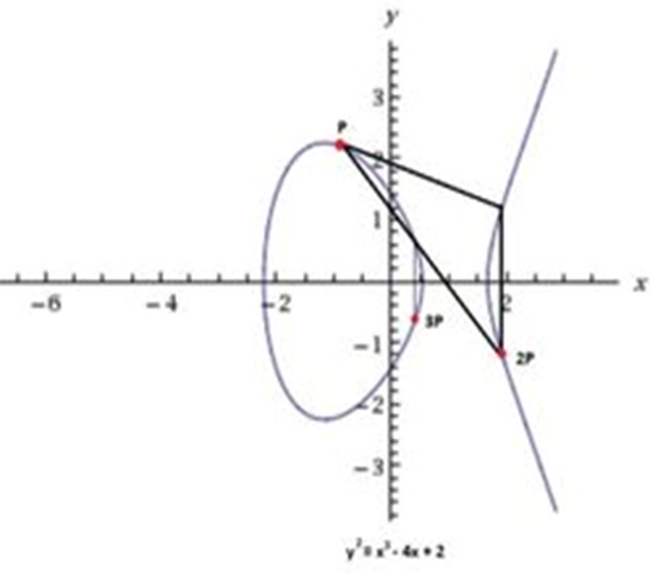
\includegraphics[scale=0.25]{pointmutiply.png}
\subsection{The Trapdoor Function}
A trapdoor function\cite{wiki:xxx}  is a function that is easy to compute in one direction, yet difficult to compute in the opposite direction without special information, called the "trapdoor". Trapdoor functions are widely used in cryptography.[9]
By using the value of R and P we have $R = k*P$ by point multiplication, we cannot calculate the value of ‘k‘. We donot have any method to find point subtraction or point division, so we cannot find $k = R/P$. After any finite number of point additions we get any another point on the curve. Thus it cannot be reversed.
The security behind the ECDSA algorithm is based on the Trapdoor Function.
In ECDSA \cite{schmid2015ecdsa}, the parameters ‘a‘ and ‘b‘ are the constants of the elliptic curve, ‘p‘ is prime modulus, and ‘N‘ is the number of points of the curve and ‘G‘ i.e a ‘reference point’. The reference point could be any point on the curve.

A private key is any generated random number (160 bits), and the public key is generated through the point of the curve through point multiplication of G with our generated private key. 
Here ‘dA‘ is the private key and ‘Qa‘ is the public key, where : $$Qa = dA * G$$ \cite{oswald2002introduction}

\subsection{Creating the Signature}
 The signature is of the size 48 bytes and is represented by values of 24 bytes each. The couple (r, s) together is the ECDSA signature.
Initially a random value ‘k‘ is generated, and we calculate the point $P=k*G$ through point multiplication. The value of P on the x-coordinate represents ‘r‘. \cite{harper1992public}

$$$$
 To calculate s, we take the SHA256 hash of the message or the text. This value (32 byte) is assigned as an integer ‘z‘. To calculate s, evaluate
  $$k^{-1} (z + dA* r) mod p$$
\subsection{Signature Verification}
To verify the ECDSA signature we only require the public key and the curve parameters. We calculate P using the equation :
$$ s^{-1}*z*G + s^{-1} *r* Qa$$
We can write
$$P = s^{-1}*z*G + s^{-1}* r * dA*G$$ 
    $$ = s^{-1} (z + dA* r) * G$$ using $$Qa = dA*G$$
We know that r is the x coordinate of $k * G$. Therefore,
$$k*G = s^{-1} (z + dA * r) *G$$

$$k = s^{-1} (z + dA * r)$$
Therefore we write
$$s = k^{-1} (z + dA *r)$$
So if the x coordinate of P and r are equal then the ECDSA signature is a valid signature.

\subsection{Security Issues in elliptic curve based signature schemes}
In \cite{vaudenay2003security}, Vaudenay listed four necessary security
conditions for DSA and ECDSA. It is necessary that the 
discrete logarithm in the subgroup spanned by G 
is difficult to reduce the possibility of computing the discrete
logarithm of the public key to receive the secret key. 
The hashing algorithm is a one-way and
a collision-resistant function that withstands forgery attacks.
Also the value of k is anonymous and cannot be guessed. \cite{WinNT22}
To verify our ECSDA signature we only require the "r" part of our signature and the public key(Qa). Also $$r=k*G$$ and $$Qa = dA*G$$. Due to the trap door function we cannot calculate "dA" or "k" through "Qa" and "R" thus it's impossible to fake a signature without the private key.

The security of the algorithm is based on the implementation. The value of ‘k‘ should be random to prevent guessing or using a timing attack or any other type of attack.
If we use the same value of k in two signatures that is the same r value then it is easy to calculate "k" using two s values of the signatures and two file hashes z and $z'$ :
 $$s- s' = k^{-1} (z + dA*r) – k^{-1} (z' + dA*r) $$
          $$= k^{-1} (z + dA*r - z'- dA*r)$$
          $$= k^{-1} (z - z')$$

So :$$ k = (z - z') / (s - s')$$
Thus the equation for s has one unknown value and can easily resolve dA :

$$dA = (s*k - z) / r$$
 Hence we can sign the files and will be recognized as a geniune file. 




\chapter{Blockchain}
The term blockchain was first described back in 1991. A group of researchers wanted to create a tool to timestamp digital documents so that they could not be backdated or changed. Further, the technique was adapted and reinvented by Satoshi Nakamoto.
Blockchain is a decentralized ,distributed, computation and information sharing platform that enables multiple authoritative domains, who do not trust each other, to cooperate, coordinate and collaborate in a rational decision making process. A blockchain is a strong database platform with strong consistency support. It records transactions between two parties efficiently and in a verifiable and permanent way[4]. It is distributed ledger which requires peer-to-peer network as well as consensus algorithms to ensure replication across nodes.The distributed ledger database is spread across several nodes on a peer-to-peer network, where each replicates and saves an identical copy of the ledger and updates itself independently. This is possible due to the lack of central authority.\cite{yinew} When a ledger update happens, each node constructs the new transaction, and then the nodes vote by consensus algorithm on which copy is correct. Once a consensus has been determined, all the other nodes update themselves with the new, correct copy of the ledger \cite{popper2016venture}\cite{brito2013bitcoin}. It is an undeniably ingenious invention which allows digital information to be distributed but not copied. Though it began with Bitcoin, it can be programmed to record not only financial transactions but virtually anything of value.\\
The blockchain is a simple yet insightful way of passing information from A to B in a fully automated and safe manner. One party to a transaction initiates the process by creating a block. This block is verified by thousands, perhaps millions of computers distributed around the net. The verified block is added to a chain, which is stored across the net, creating not just a unique record, but a unique record with a unique history. Falsifying a single record would mean falsifying the entire chain in millions of instances. That is virtually impossible. \\
Let us take a scenario \cite{WinNT23} where Alice gives Bob a coin. Now Alice has zero coins and Bob has one coin. There is no need to verify the transaction. Alice further cannot pass the same coin to Jordon, because she herself doesn't have it.

But can the same transaction be reconstructed on a digital platform?  A digital coin is simply string of binary numbers. If Alice sends Bob a digital coin through a messaging application. Now again Alice has zero coins and Bob has one coin. But Alice can certainly make copies of the coin or put the same coin online for multiple downloads. \\
So this doesn't what stops Alice from double spending. She can spent the coin twice or any finitely many times.
This is where the concept of blockchain prevails. It contains a digital ledger containing digital coin transactions. When Alice gives Bob a digital coin then the ledger records the transaction. 
But it is difficult to derive who will hold the ledger. Alice cannot hold the ledger as she may delete the transaction and claim to still own the coin for further spending. Bob too cannot hold the ledger as he could alter the value of the transactions.\cite{WinNT24}

Now they require a trusted third party who works as an intermediary say Michelle. Michelle makes sure that the ledger is updated. But can a third party always be trusted?
This is where blockchain technology steps in.
Blockchain technology is making revolutionary changes around the world. Dubai has set sights on becoming the world's first blockchain-powered state. In 2016, representatives of 30 government departments formed a committee dedicated to investigating opportunities across health records, shipping, business registration and preventing the spread of conflict diamonds. Technology giant, Samsung is creating blockchain solutions for the South Korean government which will be put to use in public safety and transport applications.[23]  The Estonian government has partnered with Ericsson on an initiative involving creating a new data center to move public records onto the blockchain. One of the world's most digitally advanced societies, in 2005 Estonia became the first state to hold elections over the Internet, and in 2014 the first state to provide e-residency. We will study electronic voting in Estonia in Section x.
\subsection{Aims of Blockchain}
Blockchain technology has the core characteristics of decentralization, accountability, and security. This technique can improve operational efficiency and save costs significantly. It's major aims are-
\begin{enumerate}
     

    \item Protocols for Commitment: Blockchain aims to ensure that every valid transaction is included.
    \item Consensus- It aims to ensure that local are consistent.
    \item Immutability and Security: It aims to be tamper-proof. Immutability, in the context of the blockchain, means that once something has been entered into the blockchain, it cannot be tampered with.
    \item Privacy and Authencity:  It is an assurance that a message, transaction, or other exchange of information is from the source it claims to be from.
    \item Peer-to-Peer : No central authority to control or manipulate it. All participant talks to each other directly. This allows for data exchange to be made directly with third-parties involvement.
\end{enumerate}

\subsection{Architecture}
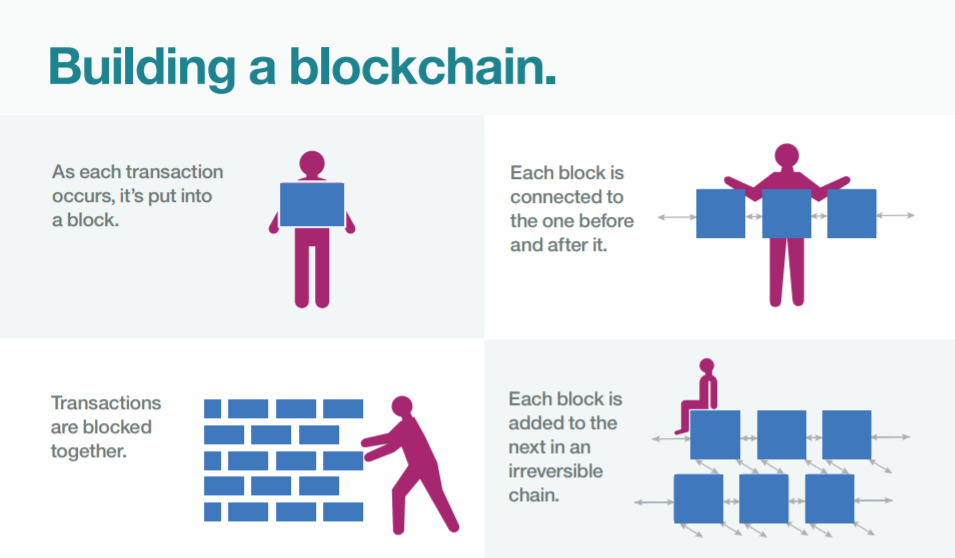
\includegraphics[scale=0.50]{voorbeeld3.png}
\\
A blockchain is a chain of blocks which contain specific database, but in a secure and genuine way that is grouped together in a peer-to-peer network . It is basically a combination of computers linked to each other instead of a central server, meaning that the whole network is decentralized.\cite{WinNT25}
Blockchain structures can be classified as-
\begin{enumerate}
\item Public blockchain architecture: It means that the access and data to the system is available to anyone who is willing to participate. The reliability of the transactions depends on the validators. A system with more validators is less likely to be tampered. A Public blockchain provides "salary" or incentives for working as a validator. Validation of transaction provides the miner cryptocurrency.
\item Private blockchain architecture: It is controlled only by users from a specific organization or authorized users who have an invitation for participation. Private blockchains are completely for private internal uses. There is a single central organization responsible for the validation process. It is not a self sustaining, flexible mechanism. The system falls without the central system.
\item Consortium blockchain architecture: This blockchain structure can consist of a few organizations. In this system procedures are set up and controlled by the preliminary assigned users.
\end{enumerate}
\subsection{MetaData in a Block}
Every single block in a blockchain contains digitally signed and encrypted transactions verified by the peers. The cryptographic security ensures that the participants can only access information on the ledger that they are authorized to see. A block has two components- Block Header and the List of transactions (in context to financial handling or bitcoin).\cite{WinNT26}
\subsubsection{Block Header}
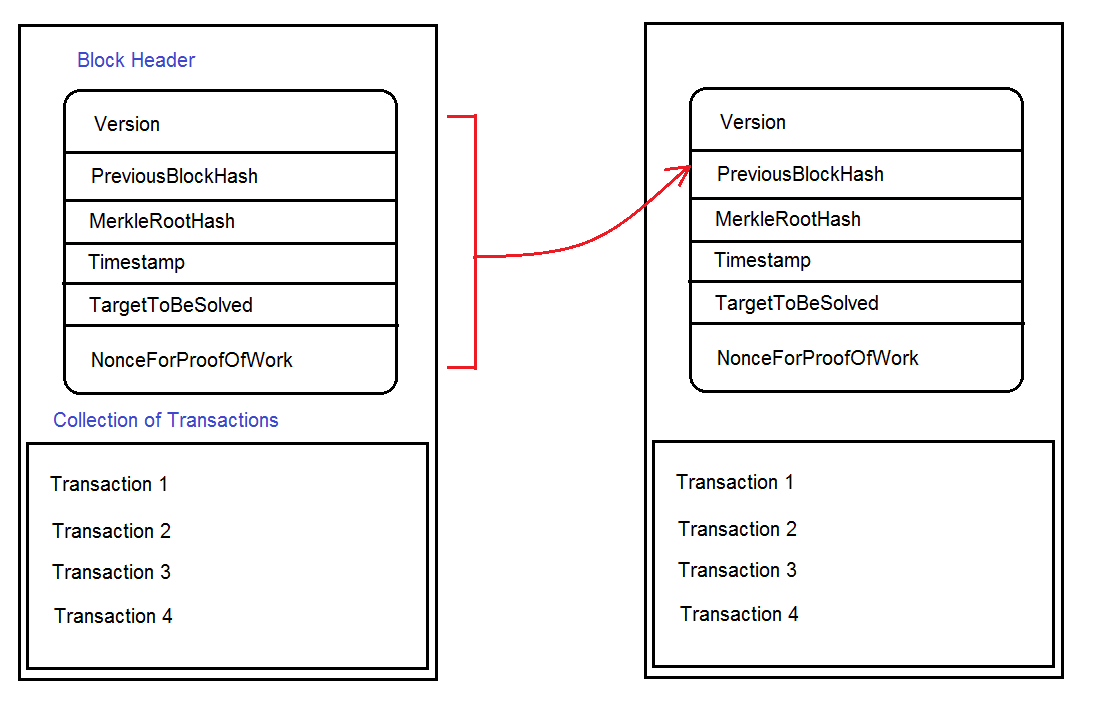
\includegraphics[scale=0.25]{chained_blocks.png}
\\
It has the following components
\begin{enumerate}
   \item Previous Block Hash- To make the blockchain tamper-proof the hash value of the previous block is used to create the new block hash.\\ $ H0 -> H1= HASH(H0) -> H2= HASH(H1)... $
   \item Mining Statistics- It is important to make the alogorithm complicated so that it is tamper-proof. For example- In bitcoin blockchain mining $HK =Hash( HK-1||T ||Nonce)$. The nonce value defines the complexity of any Hash Value HK. The MS contains the Time Stamp, nonce and difficulty.
   \item Merkle Tree Root- To secure all documents together and even if one document is tampered, the root(main) will change. It displays the property of Avalanche effect that even a slight change in data causes significant changes in the output.[25]
   \\
  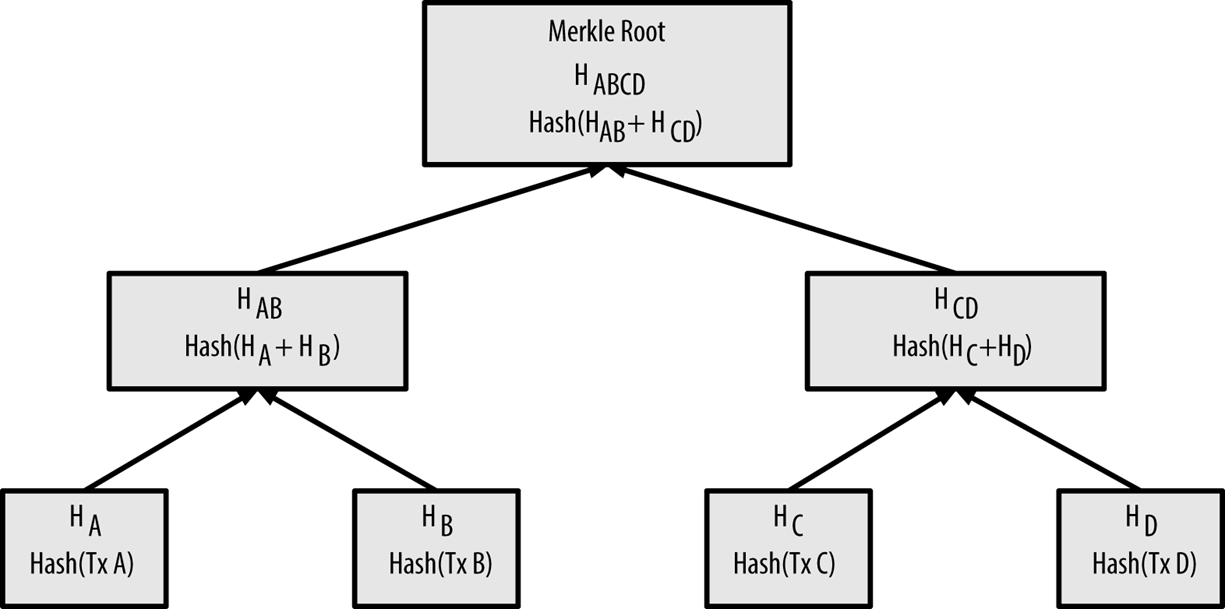
\includegraphics[scale=0.25]{Picture1.png}

\end{enumerate}
 \subsubsection{Transactions}
Each block in a blockchain contains a list of transaction performed in that block. This can be seen from the image below
\\
 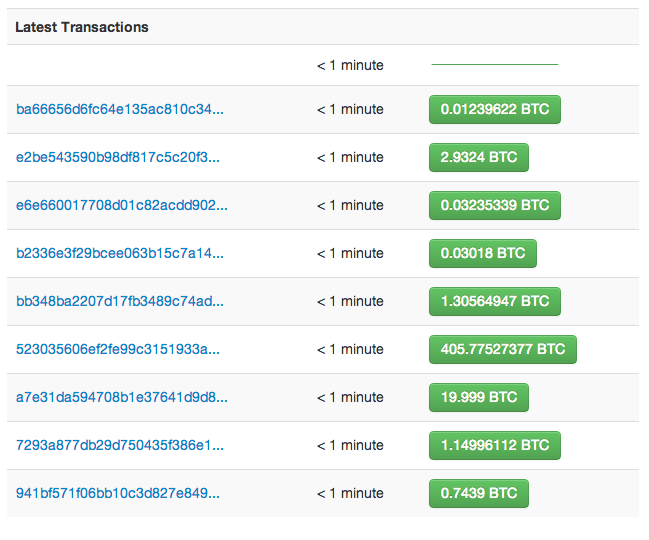
\includegraphics[scale=0.25]{blockchain-transactions.png}

\subsection{Creating a Block in a Blockchain}
A single block in a blockchain is simply a collection of data. Data is added in blockchain, by connecting it with other blocks in chronological order, creating a chain of blocks linked together. The first block in the Blockchain is called Genesis Block. Bitcoin is the oldest cryptocurrency in existance. Each block in the Bitcoin is approximately of the size 1 MB. Each block in the Bitcoin Blockchain contains 80 Kb data in Block Header and the rest as transaction history. Till now 567340 blocks of Bitcoin are mined, i.e approximately 567340 Mb is stored in the Bitcoin Blockchain.\\ \cite{WinNT27}
Now imagine files containing an amount of data (or transactions). These are isolated files and in no way linked to each other. Hence tampering any of the two files is easy. Now suppose we link the two files by assigning digital signature and merkle root to each file. We can continue adding files in this chain. These files( now blocks) are now tamperproof and even if a single file is tampered, the avalanche effect causes significant changes the signature and the merkle root. To carry an altercation in a block undetected, every single block after that block must be renewed. This is possible when the attacker has higher computational power as compared to the original network. Thus making it immutable for lengthy blockchain networks.
\\
Miners spend electricity in the form of computational energy to mine a block in a blockchain. At this phase Challenge-Response Protocol is initiated. A block is only accepted in a blockchain if it satisfy the \textit{nonce} value of the block. A nonce is an arbitrary number that can be used just once in a cryptographic communication. It is a random or pseudo-random number issued in an authentication protocol to ensure that old communications cannot be reused in replay attacks.\\
The miner that calculates an eligible signature for its block at the earliest, broadcasts the block and the signature. The legitimacy of the block is then verified by taking the string of data of the block, and hashing it to see if the output hash indeed matches the included signature. Then by the Consensus Algorithm the block is added to the  blockchain.\cite{WinNT28}

\chapter{Blockchain Voting}

The Election Commission of India developed the country’s EVMs in partnership with two government-owned companies, the Electronics Corporation of India (ECIL) and Bharat Electronics Limited (BEL). Though these companies are owned by the Indian government, they are not under the administrative control of the Election Commission. They are profit-seeking vendors that are attempting to market EVMs globally \cite{WinNT29}.  An Electronic Voting Machine consists of two Units – a Control Unit and a Balloting Unit – joined by a five-meter cable. The Control Unit is placed with the Presiding Officer or a Polling Officer and the Balloting Unit is placed inside the voting compartment. Instead of issuing a ballot paper, the Polling Officer in-charge of the Control Unit will release a ballot by pressing the Ballot Button on the Control Unit. This will enable the voter to cast his vote by pressing the blue button on the Balloting Unit against the candidate and symbol of his choice[28].  Decentralised voting systems like BitCongress and Liquid Democracy contain frameworks to enforce distributed decision making. In BitCongress, anyone with a program can plug into the system and through a specific cryptocurrency "VoteCoin" to verify votes. 
\subsection{Integrity Problem in current EVM}
We assume that the physical entity or the bulletin board is compromised. Thus we can say that the adversary has physical approach and read and write access to the voting machine. The current machine is completely susceptible to physical attacks. In Security Analysis of Indian Voting Machines \cite{wolchok2010security} (July 2010), NetIndia and University of Michigan uncovered many ways in which the Indian EVM could be tampered.\\

\textbf{Proxy replica CPUs} Due to the physical presence of the machine it is tampered. The software is burned into the CPUs by the foreign chipmakers but they are assempled in India into the control unit main boards. It is possible to substitute look-alike CPUs containing software that counts the votes dishonestly. 
\\
\textbf{Proxy Machine Units} There is no practical way to verify that the EVMs used are authentic, so it is possible to build identical looking but dishonest control units or ballot units and substitute them before an election. Since the units we examined have no effective way to verify the authenticity of the units they are paired to, replacing either unit with a dishonest one would allow the attacker to alter election results.
\\
\textbf{Altercation with Software before CPU Manufacture} The EVM report boasts “The program is burnt into the microchip on a ‘one time programmable’ basis (OTP) and once burnt it cannot be read, copied out, altered and re-fed into the chip at all” Thus the software is prone to tampering as there is no method to verify it’s integrity. If the software is tampered there is no provision for examining it’s integrity. There is a huge chance of a possible backdoor through current technology.\\
\textbf{Altercation with Machine State} It is possible to attach additional hardware to the control unit’s circuit board, an attacker can directly read and write the chips that record the votes. The design protect or authenticate data stored in the machine cannot be verified for tampering.\\ \cite{agarwala2006report}
\subsection{Elements of the Proposed System}
We consider for the sake of neutrality the voting authorities to be comprised and have read and write access to the voting machine. Initially, it requires voter information to be collected.
We require an identification device, we assume it to be a fingerprint scanner and a bio-metric device. These are then instated in an inbuilt blockchain containing voter information. If the system deems the voter eligible to vote the only he can proceed.
Finally, the voting process is commenced and a seperate blockchain is maintained to store the recorded votes. Then the votes are tallied.
\subsection{Voter Information and Registration Blockchain}
Months before voting day, personal information of voters is saved. This information is used verify the voter's eligiblity during authentication process. This is similar to the AADHAR\cite{WinNT30} registration. Registration booths are setup where election officers collect details of voters. This includes their personal information, fingerprint and biometric. This data is then stored in a private blockchain. The integrity of the registration is based upon the election officers.\\
The Merkle Root as discussed in Section 4.3.1  used in the blockchain make the information tamper proof. It is considered as a hypothetical seal which binds the data. The data once entered cannot be tampered.
\subsection{Voting Phase}
In this section we will discuss the algorithm for our voting machine, voting phase and vote tallying.

\subsubsection{Implementation Setup}
There are presently three frameworks for implementing a smart contract for a voting application blockchain.\\
1) Exonum: Exonum\cite{WinNT33} enables you to build decentralized, secure and reliable blockchain applications. It is designed to allow people, companies and governments to design custom private or permissioned blockchains that benefit from the unmatched security of public blockchains. Exonum brings all the advantages of a true blockchain — auditability, transparency, and unparalleled security — and combines them with privacy, efficiency and controllability[36]. Previously, Rust was the only programming language in the current version, which used to limit construct in the language. With the latest update, Exonum has introduced Java-bindings and platform-independent interface description to make Exonum more developer-friendly.\\
2) Truffle Suite: Truffle Suite contains Truffle, Ganache and Drizzle Platforms. Truffle is an all in one Ethereum Decentralized application development environment. It provides a testing framework for Ethereum Network\cite{WinNT31}. It is the most used Integrated Development Environment.\\

The construction of the voting machine is through the Truffle Framework. It allows us to built our own decentralized application on Ethereum network. The ethereum package is an open-source, public, blockchain-based computing platform and OS featuring smart contract. The Ganache package on the Truffle framework builts a local in-memory blockchain. It also provides 10 external ethereum accounts for testing our Ethereum Blockchain. The Truffle framework also provides a testing console to prevent contract disruption and ether expenditure. It allows us to built the client-side application through it. We are using The Metamask extension\cite{WinNT32}, which allows our node to interact with our local blockchain without running a full Ethereum node. The version of solidity in our truffle framework is 0.5.0.
\subsubsection{Cryptographic Setup} The system works over Elliptic Curve Digital Signature Algorithm. The decisional Diffie-Hellman assumption[34] holds over the system, that is "The two probability distribution {($g^a$,$g^b$,$g^{ab}$): a, b are randomly and independently chosen from $Z^*_q$} and {($g^a$,$g^b$,$g^c$): a,b,c are randomly and independently chosen from $Z_q$} are computationally indistinguishable in the security parameter n= log(q)."\\
The system is publicly accessible and can be functional on any  Ethereum node or any web browser with a bridge extension. We are using the Metamask extension on the chrome web browser. The system incorperates voter auditing to achieve end-to-end verifiability. We include one public and one private blockchain in our system. The private blockchain contains the data of the voters. The public blockchain contains the candidates participating in the election. It also stores the votes recived by the candidates in the election and  This also marks a flag boolean value that the voter has already voted or not in the election. Whenever a vote is casted, the blockchain creates and mines a new block in the blockchain.\\
Here we initiate our smart contract with only candidates. The HTML format of the page allows editing of the vote which was not possible in conventional EVM machines(April 2019). We are using Truffle Ganache framework. This gives us ten accounts with test ether. They have a unique address and private key. Any account among them can be imported in our blockchain using the Metamask Extension. The key generation algorithm executes the Cramer-Shoup method.
\\
\\
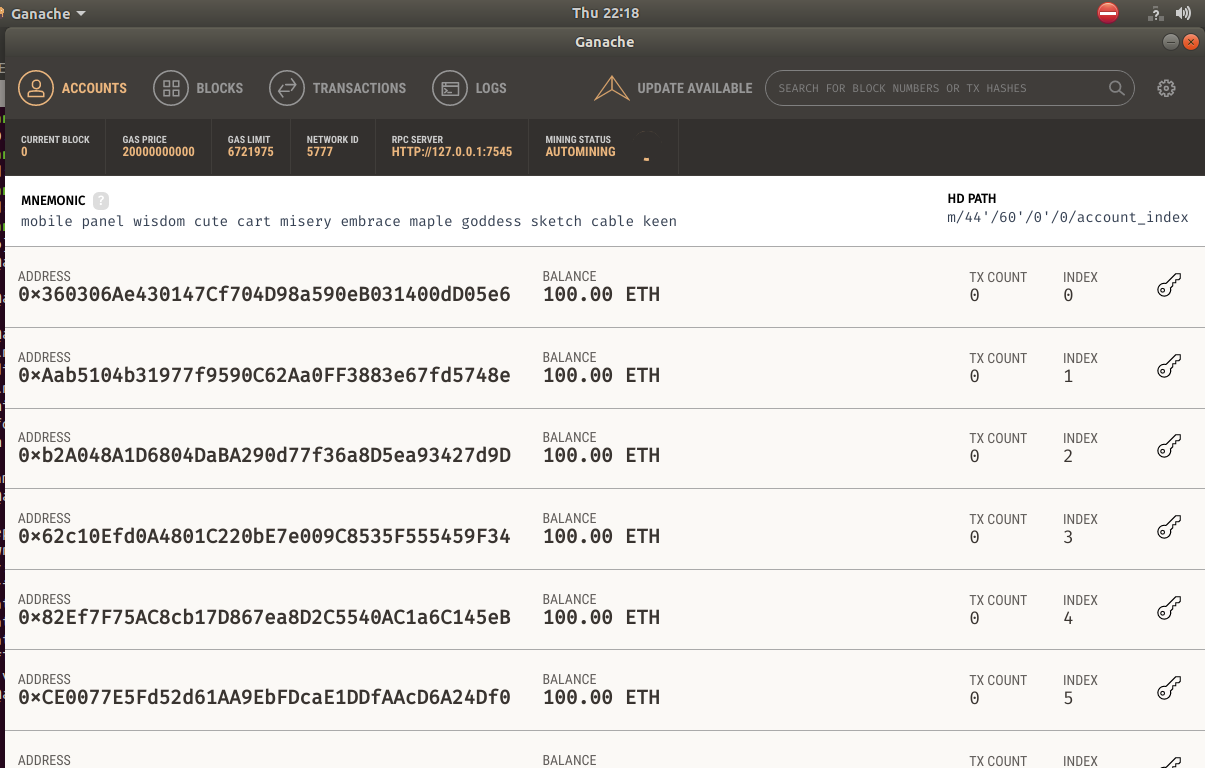
\includegraphics[scale=0.45]{ganache1.png}
\\
\\
The Truffle Framework comes with the Solidity platform. Solidity is an object-oriented programming language for writing smart contracts. It implements our smart contract in the blockchain. A smart contract is a programmable bond of sorts, a fair judge capable of managing a financial transaction between various parties and autonomously resolving a dispute \cite{dannen2017introducing}. For our voting machine we have constructed a smart contract that along with including Candidate information contains a set of restriction for the voters to prevent double voting. The truffle console also allows us to saves the accounts that have already participated in the election. We are using Sublime Text Editor to write our code.
\\
\\
\begin{verbatim}
    pragma solidity ^0.5.0;

contract Election {
    // Model Canditate
    struct Candidate {
        uint id;
        string name;
        uint voteCount;
    }

    // Storing Accounts that have already participated in the election
    mapping(address => bool) public voters;

    // Reading and writing candidate information
    mapping(uint => Candidate) public candidates;

    // Storing the number of Candidates
    uint public candidatesCount;

    event votedEvent (
        uint indexed _candidateId
        );

        constructor() public {
            addCandidate("Candidate 1");
            addCandidate("Candidate 2");
        }

        function addCandidate (string memory _name) private {
            candidatesCount ++;
            candidates[candidatesCount] = Candidate(candidatesCount, _name, 0);
        }

        function vote (uint _candidateId) public {
            // require that they haven't voted before
            require(!voters[msg.sender]);

            // require a valid candidate
            require(_candidateId > 0 && _candidateId <= candidatesCount);

            // record that the voter has voted
            voters[msg.sender] = true;

            // update candidate vote Count
            candidates[_candidateId].voteCount ++;

            // trigger voted event
        emit votedEvent(_candidateId);
        }


}              
\end{verbatim}
\\
\\
This smart contract allows us define the structure of the candidate where the "id" and "voteCount" are unsigned integers. The "name" of the candidate is to be defined as a string value. Mapping in solidity is similar to dictionaries in Python. It consists of two parts KEYTYPE and VALUETYPE. In our test voting interface we save the accounts that have already voted in boolean values. This need not be done in realtime voting. A separate private blockchain containing voter information and boolean flags for accounts/voters that have already voted obviates this step. Also each candidate participating in the election is provided a unique id as defined in the struct. The candidate struct is then initialized with the candidate id with each candidate beginning from null votes. Also it adds some features for console voting. If we deploy the contract in the console the contract returns an error if an unvalid candidate is selected. The contract makes sure that all the ideals of voting are ensured. Each voter only votes once and the candidate with the highest votes wins.
\\
Now for our client-side application we configure a JavaScript file. This file provides an interface for our web configurations. Functions that will be deployed in the contract are defined in this file. This app is deployed when the client-side application is initialized. We use WEB3 to connect our application and blockchain through our METAMASK extension. "web3.js" is a collection of libraries which allows us to interact with a local Ethereum node, using an HTTP, WebSocket or IPC connection. It allows us to transfer ether from one account to another. It simply turns our browser into a blockchain cooperative setup. We setup our function such that our current web3 provider works in our application. We can also setup an instance as a localhost from our Ganache local network.  When we completely setup our required connections we initialize our smart contract in the application. We use JSON to transmit our data between the server and the web application. This is possible through the BROWSERSYNC Package from Truffle Box.
\\

\\
Next, we specify our function to react to a voted event. In realtime voting we keep this page private and allow only authorized access. But for simplicity purposes, we refresh the page any time a voting event is triggered. This shows the updated value of the total votes accumulated by each candidate during the reign of the election. We now project data on our page through our contract. To accomplish this we use the render function.  The render function is similar to the Body command in HTML. In our voting interface we require the candidates contesting the election. All the data deployed here is apprehended through our smart contract. Also we display the account through which we are logged in METAMASK. In realtime voting each voter has only one account. This account may be called as Voter Unique Identification Number.
\\

\\
We cannot access our candidates directly due to the intricate structure of blockchain. So, we write a loop according to the number of candidates specified in our contract. This is just our basic template regarding how much information we want our contract to display in the client-side application. The private functions in the contract remain unaccessable thoughout the application and can only be changed if the contract is renewed. 
\\

\\
Finally we want our client-side application to cast their vote. It requires a valid candidate Id and checks that the account. The vote function deployed in contract insures that the votes are updated and account used to carry that function is recorded.

\subsubsection{Client-Side Setup and Voting}
 After all these steps and making some changes in the HTML file in text editor, we run this program through our terminal. We are using chrome browser with a METAMASK extension logged in. This allows us to interact with our blockchain. The BROWSERSYNC allows us to host our local network. This is what our page looks like. We allow our election to have more than one candidate by renewing our smart contract.The application also shows us the account through which we have logged in. In realtime voting it can be the voter's information submitted in the private blockchain.
 \\
 \\
 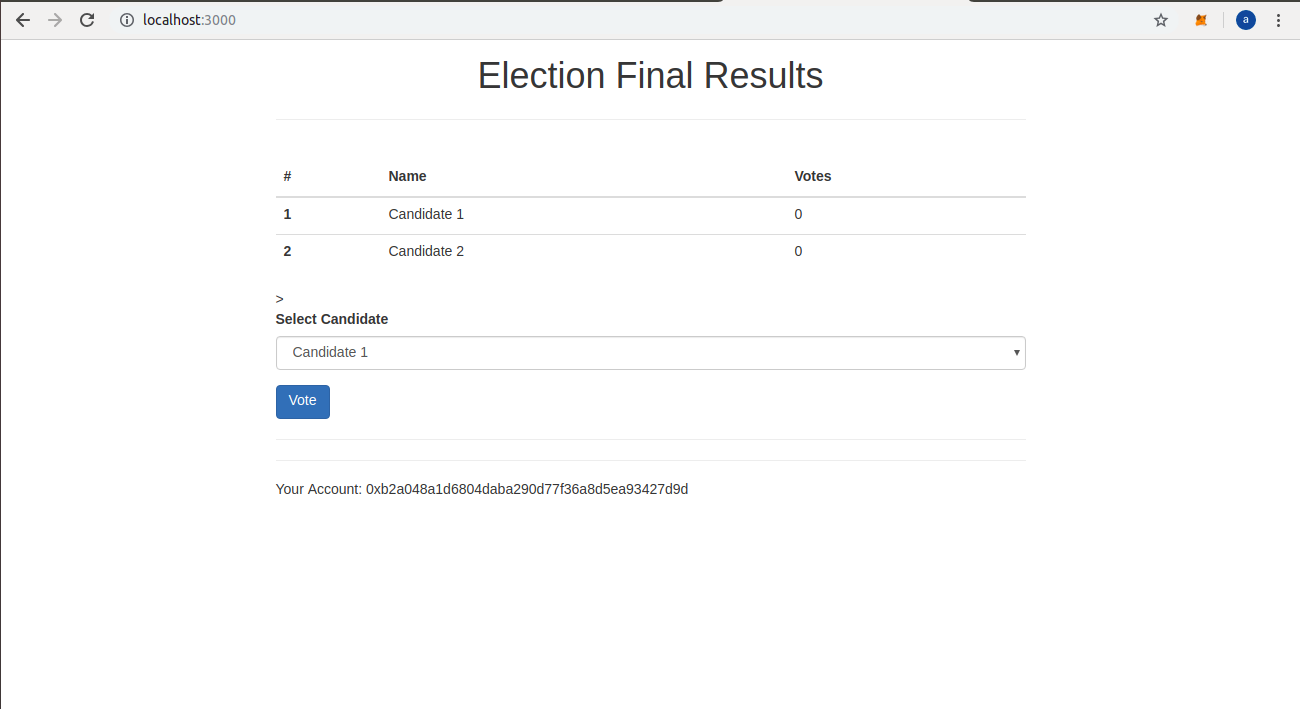
\includegraphics[scale=0.45]{chrome1.png}
 \\
 \\
 We have created a simple client application page. The candidates displayed in this page are specified in the contract. We have created the vote and result functions on the same page. Seperate pages can be constructed and the result page can be made private.
 \\
 \\
 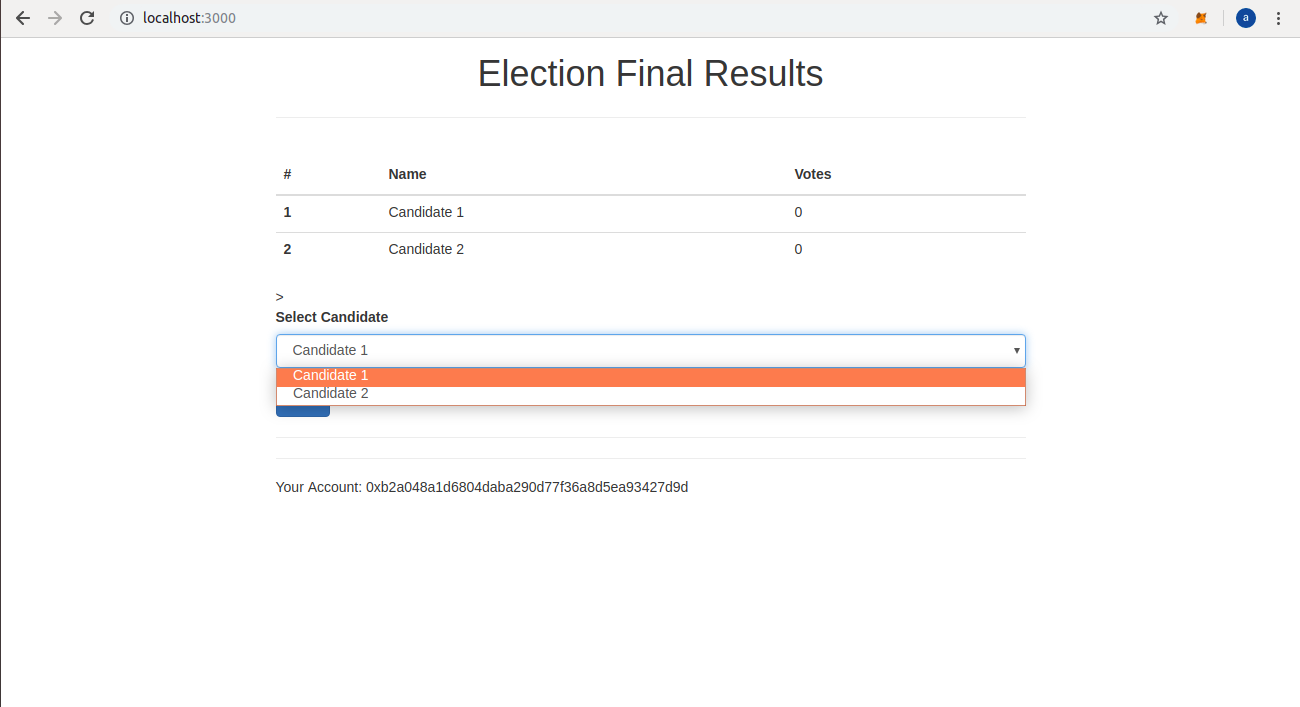
\includegraphics[scale=0.45]{chrome2.png}
 \\
 We are using the Ethereum network. The construction of the blockchain is freely possible but writing in it costs energy. The computational energy in Ethereum is termed as GAS. Gas is spent when a blockchain is operated at the local network. But voting in the Main Ethereum Network blockchain costs Ether. 
 \\
 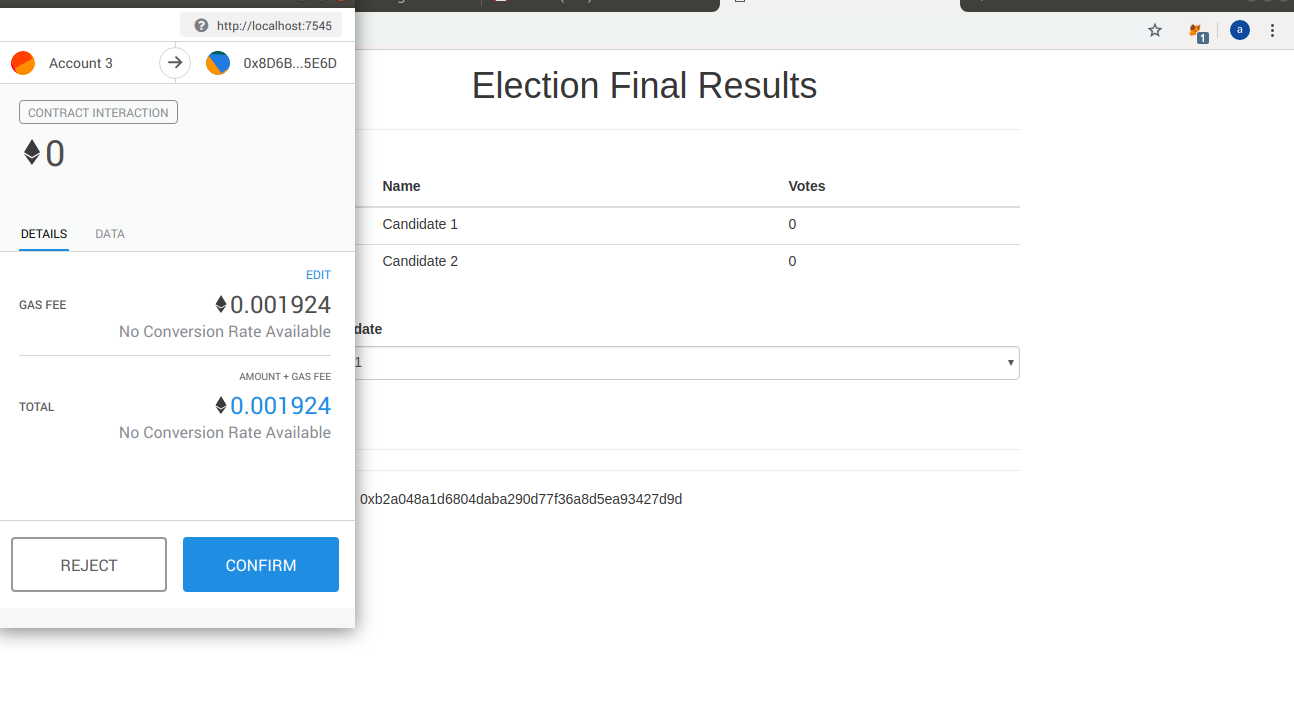
\includegraphics[scale=0.45]{chrome3.png}
 \\
 Thus any smart electronic device with an internet connection from anywhere can be used by any eligible voter to cast his vote. Now after casting the vote, the data is proceeded to be verified by the corresponding node of the smart contract. The vote must be agreed upon by the majority corresponding district node through the guidelines of the smart contract. All the transactions that are received and verified in the corresponding block time are deployed onto the blockchain.\\
 \\
 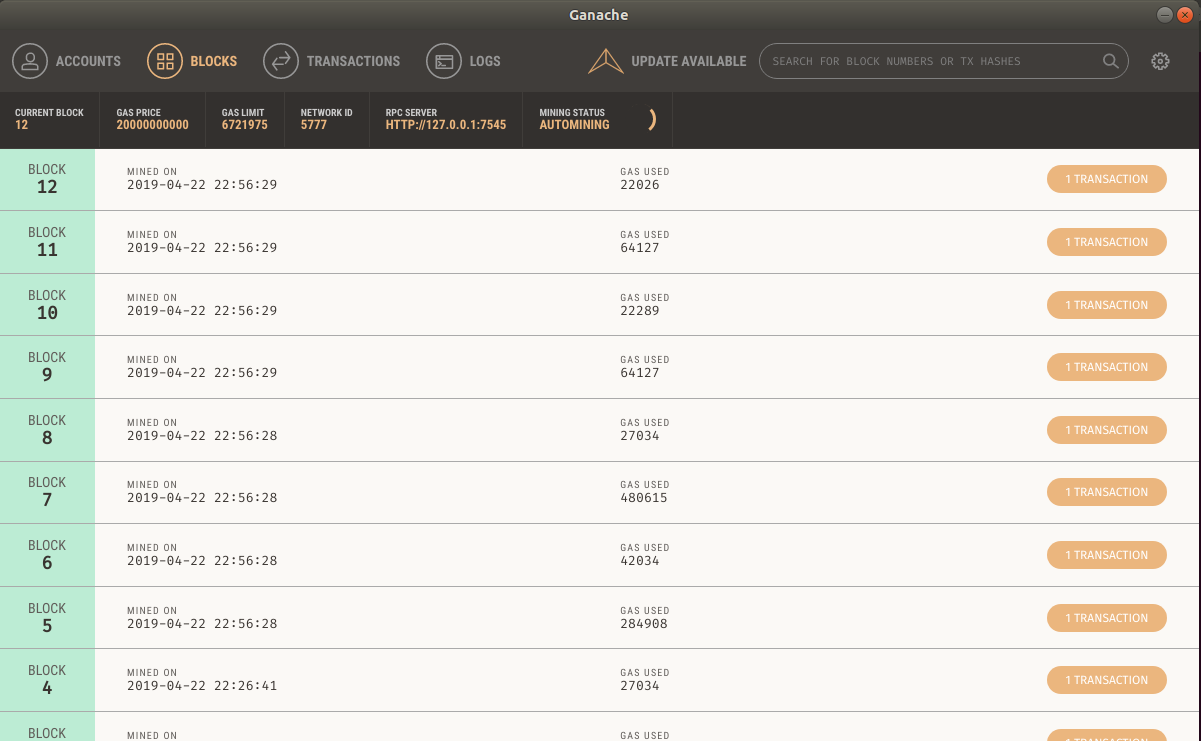
\includegraphics[scale=0.45]{ganache3.png}













\subsection{Security Concerns in Blockchain Voting}
Each individual is identified and authenticated by the system by electronic ID and their national identification stored in the private blockchain. Any individual attempting to vote for multiple people cannot proceed further due to the double voting clause in the smart contract. The biometric scan in the national identification prevents multiple accounts of the same user. 
But all this requires continuous electricity and interrupted internet facilities which may not be available to everyone in every part of the country.  Also during the setup of private blockchain for voter information requires energy resources.
Beside the energy exploitation issues in blockchain there are few security issues in Blockchain. Specially countries with large population require large storage capacity. The security of the vote is proportional to the integrity of the software. Any minor fault in the software can lead to major catastrophe like vote disruption or compromise of voter privacy. It should be added that not only championing the election in favour of a particular candidate is tampering but also disrupting the general flow of the election. Precarious softwares and equipment when used on national platform can cause major distruption and uncertainty among the general public regarding the legitimacy of the election's outcome. It also compromises the ballot secrecy that is one of the main objective of voting. One of the most serious threats is vulnerability to collusion. Malwares may not exist in system but can be present in the user's platform that may lead to vote tampering or even cyberthreats.
The Consensus algorithm is applied on each ballot to be stored in the blockchain. But it can be possible that a majority of nodes of the organisation may accept and mine fraud ballots leading to tampered results. Also outsider influence such as nation states or terrorist organizations may infiltrate the network servers, planting tampered software to creating collusion to distrupt the election remotely. These attacks may not be even detected by The Election Committee.
Future technologies like Quantum computing are compatible to break cryptographic codes posing a threat to blockchain technology. It uproots the basic security assumption of elliptic curve cryptography, that is the factorization large numbers. Cryptographic algorithms called quantum-safe or post-quantum algorithms are now being experimented that cannot be attacked by quantum computers. 
\section{Conclusion}
 Blockchain is a convenient and secure way to vote online. It will increase vote turnout and will create records that are secure and difficult to tamper. It will encourage voters to participate in the election through the comfort of their homes. The major benefit of blockchain voting is the transparency of votes. It allows the votes to be tracked by many different sources while still maintaining the privacy of the voters. But like every technology it still has some limitations that should not be overlooked. Infusing quantum-safe algorithms with the blockchain technology may be a step further to achieve the goal of an ideal voting machine. It removes the prospect of any physical tampering but it should be protected from cyber attacks on it's software.

\bibliography{references}
\bibliographystyle{ieeetr}



\appendix
\chapter{Contract Test Codes}
\begin{enumerate}
    \item To check that the application initialises with the candidates specified.\\
    \\
    \begin{verbatim}
    var Election = artifacts.require("./Election.sol");

contract("Election", function(accounts) {
        var electionInstance;

        it("initializes with two candidates", function() {
                return Election.deployed().then(function(instance) {
                        return instance.candidatesCount();
                }).then(function(count) {
                        assert.equal(count, 2);
                });
        });  
}
    \end{verbatim}
\\
    \item To check that it assigns correct values to candidates.\\
    \\
    \begin{verbatim}
    var Election = artifacts.require("./Election.sol");

contract("Election", function(accounts) {
        var electionInstance;
        it("initializes the candidates with the correct values", function() {
                return Election.deployed().then(function(instance) {
                        electionInstance = instance;
                        return electionInstance.candidates(1);
                }).then(function(candidate) {
                        assert.equal(candidate[0], 1, "contains the correct id");
                        assert.equal(candidate[1], "Candidate 1", "contains the correct name");
                        assert.equal(candidate[2], 0, "contains the correct vote count");
                        return electionInstance.candidates(2);
                }).then(function(candidate) {
                        assert.equal(candidate[0], 2, "contains the correct id");
                        assert.equal(candidate[1], "Candidate 2", "contains the correct name");
                        assert.equal(candidate[2], 0, "contains the correct vote count");

                });
        });
}        
    \end{verbatim}
\\
    \item To check that it does not allows double voting.\\
    \\
   \begin{verbatim}
    var Election = artifacts.require("./Election.sol");

contract("Election", function(accounts) {
        var electionInstance;
        it("initializes the candidates with the correct values", function() {
        it("throws an exception for double voting", function() {
        return Election.deployed().then(function(instance) {
            electionInstance = instance;
            candidateId = 2;
            electionInstance.vote(candidateId, { from: accounts[1] });
            return electionInstance.candidates(candidateId);
        }).then(function(candidate) {
            var voteCount = candidate[2];
            assert.equal(voteCount, 1, "accepts first vote");
            // Try to vote again
            return electionInstance.vote(candidateId, { from: accounts[1] });
        }).then(assert.fail).catch(function(error) {
            assert(error.message.indexOf('revert') >= 0, "error message must contain revert");
            return electionInstance.candidates(1);
        }).then(function(candidate1) {
            var voteCount = candidate1[2];
            assert.equal(voteCount, 1, "candidate 1 did not receive any votes");
            return electionInstance.candidates(2);
        }).then(function(candidate2) {
            var voteCount = candidate2[2];
            assert.equal(voteCount, 1, "candidate 2 did not receive any votes");
        });
    });
}

   \end{verbatim}
   
   \item To check that it allows only valid candidates to cast their vote.
   \begin{verbatim}
   var Election = artifacts.require("./Election.sol");

contract("Election", function(accounts) {
        var electionInstance;
   
         it("throws an exception for invalid candidates", function() {
        return Election.deployed().then(function(instance) {
            electionInstance = instance;
            return electionInstance.vote(99, { from: accounts[1] })
        }).then(assert.fail).catch(function(error) {
            assert(error.message.indexOf('revert') >= 0, "error message must contain revert");
            return electionInstance.candidates(1);
        }).then(function(candidate1) {
            var voteCount = candidate1[2];
            assert.equal(voteCount, 1, "candidate 1 did not receive any votes");
            return electionInstance.candidates(2);
        }).then(function(candidate2) {
            var voteCount = candidate2[2];
            assert.equal(voteCount, 0, "candidate 2 did not receive any votes");
        });
    });
} 
 \end{verbatim}
\chapter{Functions defined in the application}

\begin{verbatim}
    

App = {
  web3Provider: null,
  contracts: {},
  account: '0x0',
  hasVoted: false,

  init: function() {
    return App.initWeb3();
  },

  initWeb3: function() {
    // TODO: refactor conditional
    if (typeof web3 !== 'undefined') {
      // If a web3 instance is already provided by Meta Mask.
      App.web3Provider = web3.currentProvider;
      web3 = new Web3(web3.currentProvider);
    } else {
      // Specify default instance if no web3 instance provided
      App.web3Provider = new Web3.providers.HttpProvider('http://localhost:7545');
      web3 = new Web3(App.web3Provider);
    }
    return App.initContract();
  },

  initContract: function() {
    $.getJSON("Election.json", function(election) {
      // Instantiate a new truffle contract from the artifact
      App.contracts.Election = TruffleContract(election);
      // Connect provider to interact with contract
      App.contracts.Election.setProvider(App.web3Provider);

      App.listenForEvents();

      return App.render();
    });
  },

  // Listen for events emitted from the contract
  listenForEvents: function() {
    App.contracts.Election.deployed().then(function(instance) {
      // Restart Chrome if you are unable to receive this event
      // This is a known issue with Metamask
      // https://github.com/MetaMask/metamask-extension/issues/2393
      instance.votedEvent({}, {
        fromBlock: 0,
        toBlock: 'latest'
      }).watch(function(err, event) {
        console.log("event triggered", event)
        // Reload when a new vote is recorded
        App.render();
      });
    });
  },

  render: function() {
    var electionInstance;
    var loader = $("#loader");
    var content = $("#content");

    loader.show();
    content.hide();

    // Load account data
    web3.eth.getCoinbase(function(err, account) {
      if (err === null) {
        account = web3.eth.defaultAccount;
        $("#accountAddress").html("Your Account: " + account);
      }
    });

    // Load contract data
    App.contracts.Election.deployed().then(function(instance) {
      electionInstance = instance;
      return electionInstance.candidatesCount();
    }).then(function(candidatesCount) {
      var candidatesResults = $("#candidatesResults");
      candidatesResults.empty();

      var candidatesSelect = $('#candidatesSelect');
      candidatesSelect.empty();

      for (var i = 1; i <= candidatesCount; i++) {
        electionInstance.candidates(i).then(function(candidate) {
          var id = candidate[0];
          var name = candidate[1];
          var voteCount = candidate[2];

          // Render candidate Result
          var candidateTemplate = "<tr><th>" + id + "</th><td>" + name + "</td><td>" + voteCount + "</td></tr>"
          candidatesResults.append(candidateTemplate);

          // Render candidate ballot option
          var candidateOption = "<option value='" + id + "' >" + name + "</ option>"
          candidatesSelect.append(candidateOption);
        });
      }
      return electionInstance.voters(web3.eth.defaultAccount);
    }).then(function(hasVoted) {
      // Do not allow a user to vote
      if(hasVoted) {
        $('form').hide();
      }
      loader.hide();
      content.show();
    }).catch(function(err) {
      console.warn(err);
    });
  },

  castVote: function() {
    var candidateId = $('#candidatesSelect').val();
    App.contracts.Election.deployed().then(function(instance) {
      return instance.vote(candidateId, { from: web3.eth.defaultAccount });
    }).then(function(result) {
      // Wait for votes to update
      $("#content").hide();
      $("#loader").show();
    }).catch(function(err) {
      console.error(err);
    });
  }
};

$(function() {
  $(window).load(function() {
    App.init();
  });
});
      
\end{verbatim}
\cite{WinNT55}
  
\end{enumerate}



\end{document}
